% Warm-up document for high-school mathematics content (see
% prisma/math-templates.ts). Tectonic runs with --only-cached, so every
% package, TikZ library and font size used by those templates must be
% exercised here at image build time.
\documentclass[11pt,a4paper]{article}
\usepackage{iftex}
\usepackage[turkish,shorthands=:!]{babel}
\usepackage[margin=1.6cm]{geometry}
\usepackage{amsmath,amssymb,amsthm,mathtools}
\usepackage{multicol}
\usepackage{enumitem}
\usepackage{tikz}
\usetikzlibrary{
  babel, angles, quotes, calc, arrows.meta, trees, positioning,
  intersections, through, patterns, decorations.markings, 3d
}
\usepackage{tkz-euclide}
\usepackage{pgfplots}
\usepgfplotslibrary{fillbetween}
\pgfplotsset{compat=1.18}

\begin{document}

{\tiny tiny $x^2$} {\scriptsize scriptsize $x^2$} {\footnotesize footnotesize $x^2$}
{\small small $x^2$} normal $x^2$ {\large large $x^2$} {\Large Large $x^2$}
{\LARGE LARGE} {\huge huge}
\textbf{Kalın $\mathbf{x}$} \textit{İtalik} \emph{vurgu} \texttt{mono}
Türkçe: ğ ü ş ı ö ç Ğ Ü Ş İ Ö Ç — â î û
$\alpha\beta\gamma\theta\pi \sqrt{2} \frac{3}{5} \tfrac{4}{3} \dfrac12 \le \ge \perp \parallel \angle \triangle \overline{AB} \widehat{ABC} \mathbb{R}$

\begin{multicols}{2}
\begin{enumerate}[label=\Alph*)]
  \item bir \item iki
\end{enumerate}

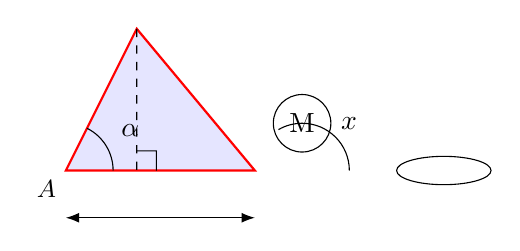
\begin{tikzpicture}[scale=0.6]
  \coordinate (A) at (0,0);
  \coordinate (B) at (4,0);
  \coordinate (C) at (1.5,3);
  \coordinate (H) at ($(A)!(C)!(B)$);
  \draw[thick, fill=blue!10, draw=red] (A) -- (B) -- (C) -- cycle;
  \draw[dashed] (C) -- (H);
  \pic[draw, angle radius=2.5mm] {right angle = C--H--B};
  \pic[draw, "$\alpha$", angle eccentricity=1.6, angle radius=6mm] {angle = B--A--C};
  \node[below left, font=\small] at (A) {$A$};
  \node[label=right:{$x$}, circle, draw] at (5,1) {M};
  \draw[{Latex}-{Latex}] (0,-1) -- (4,-1);
  \draw (6,0) arc[start angle=0, end angle=120, radius=1];
  \draw (8,0) ellipse (1 and 0.3);
\end{tikzpicture}

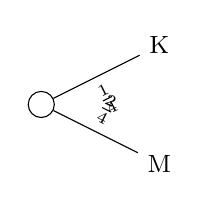
\begin{tikzpicture}[grow=right, sloped, every node/.style={font=\small}]
  \node[circle, draw] {}
    child { node {M} edge from parent node[above] {$\frac{2}{4}$} }
    child { node {K} edge from parent node[below] {$\frac{1}{4}$} };
\end{tikzpicture}
\end{multicols}

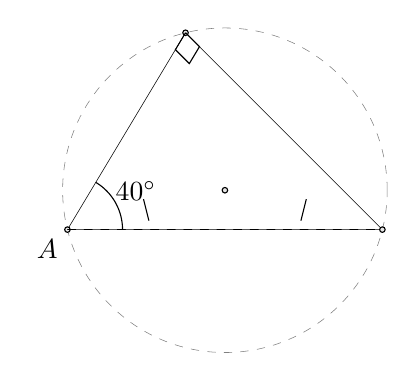
\begin{tikzpicture}
  \tkzDefPoints{0/0/A, 4/0/B, 1.5/2.5/C}
  \tkzDefCircle[circum](A,B,C) \tkzGetPoint{O}
  \tkzDrawCircle[dashed](O,A)
  \tkzDrawPolygon(A,B,C)
  \tkzDrawPoints(A,B,C,O)
  \tkzLabelPoints[below left](A)
  \tkzMarkAngle[size=0.7](B,A,C)
  \tkzLabelAngle[pos=1](B,A,C){$40^\circ$}
  \tkzMarkSegments[mark=|](O,A O,B)
  \tkzMarkRightAngle(A,C,B)
  \tkzDrawSegment[dashed](A,B)
\end{tikzpicture}

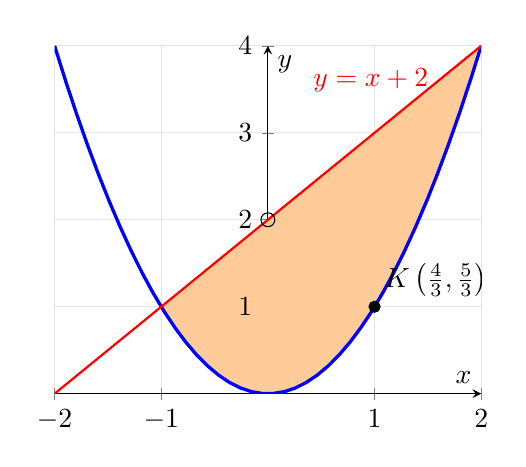
\begin{tikzpicture}
  \begin{axis}[
    axis lines=middle, xlabel={$x$}, ylabel={$y$},
    grid=both, grid style={gray!20},
    width=7cm, height=6cm,
  ]
    \addplot[name path=f, very thick, blue, domain=-2:2, samples=40] {x^2};
    \addplot[name path=g, thick, red, domain=-2:2] {x + 2} node[pos=0.9, left] {$y=x+2$};
    \addplot[orange!40] fill between[of=f and g, soft clip={domain=-1:2}];
    \addplot[only marks, mark=*] coordinates {(1,1)};
    \addplot[only marks, mark=o, mark size=2.5pt, fill=white] coordinates {(0,2)};
    \node[above right] at (axis cs:1,1) {$K\left(\tfrac43,\tfrac53\right)$};
  \end{axis}
\end{tikzpicture}

\end{document}
